\chapter{Avant de commencer}

\section{Comment lire ce cours}
\subsection{Pré requis}
Pour profiter pleinement de ce cours, il faut :
\begin{itemize}
\item Disposer d'un Mac (récent) tournant sous OS X Yosemite (10.10),
et savoir s'en servir un minimum.
\item Être \emph{persévérant}, \emph{rigoureux} et \emph{logique}.
\item Ne pas faire une allergie à la langue de Shakespeare
(On croirais entendre mourir un auvergnat, je sais ;).
\item Un petit bagage mathématique, en gros les acquis du collège.
La programmation ne nécessite pas plus de connaissances mathématiques.
(Excepté l'informatique théorique, mais ce n'est pas là mon propos.) 
\end{itemize}

\subsection{De le méthode}
Avant d'entrer dans le vif du sujet,
un peu de méthodologie (même si c'est barbant).


Ce cours essaye d'être accessible au débutant,
mais il est important d'acquérir de bonnes bases
pour pouvoir comprendre la suite.
Certains chapitres peuvent être très denses,
donc n'hésitez pas à les relire plusieurs fois.


En effet, pour bien acquérir un cours, il faut :
\begin{description}
\item[Le Comprendre]
car on ne peut pas retenir et appliquer un cours sans le comprendre.
\item[Le Reprendre] plusieurs fois,
car une bonne mémorisation ne peut se faire qu'à ce prix.
\item[Le Pratiquer],
c'est à dire ne pas copier coller bêtement mon code sans le comprendre.
C'est en \emph{cherchant} que l'on tire le meilleur profit d'un exercice :
\emph{Tiens, j'ai essayé ça, Pourquoi cela n'a il pas marché ?}
Essayez d'être \emph{curieux}, de pousser mes exemples dans leurs retranchements,
de les \emph{modifier}. Ne jetez pas l'éponge si vous n'avez pas d'idée après 5 secondes,
ou si votre première idée ne marche pas.
Enfin, essayez d'exécuter pas à pas votre code dans votre tête,
pour vérifier qu'il fait bien ce que vous aviez l'intention de faire.
\end{description}
Cette méthode de travail est la \emph{meilleure}, d'expérience d'élève en classe préparatoire
(NB : Cette méthode marche à tous les niveaux d'études).
\paragraph{Compléments :}
Certaines sections dont le titre commence par complément
ne sont pas indispensables à la suite du cours.
Elles sont là pour la culture, ou par soucis d'exhaustivité,
ou encore s'addressent à un publique particulier.
Vous pouvez les laisser de coté lors d'une première lecture.
\subsection{Risque d’évolution}
Ce cours est susceptible d'évoluer rapidement,
du fait que Swift n'est pas encore stabilisé.

Le site
\TSwiftUrl{https://github.com/ksm/SwiftInFlux/blob/master/README.md}{SwiftInFlux}{SwiftInFlux} 
répertorie les évolutions de Swift,
y compris celles qui ne sont encore que envisagées.
\section{Quelques notions sur le fonctionnement d'un ordinateur}
\subsection{Qu'est-ce qu'un ordinateur ?}
Qu'est-ce qu'un ordinateur ?
Avant tout une machine qui manipule des données
(par exemple la photo de votre chat, chien, petit-neveu ;
le site Web que vous consultez, ou le résultat d'une expérience du LHC),
et cela selon un programme qui peut être changé,
c'est à dire que le \emph{programme est lui même une sorte de donnée}.

Ainsi, les organes les plus importants d'un ordinateur sont
sa mémoire, qui contient les données, et le processeur,
qui exécute le programme, lui aussi stocké en mémoire, puisque c'est une donnée.

Ensuite, un ordinateur possède aussi des entrées et des sorties (E/S ou I/O, en anglais),
qui lui permettent de communiquer avec le reste du monde
(la carte graphique qui affiche ce texte à l'écran,
la carte réseau qui permet de charger des pages Web,
la carte son, un clavier, une souris...).

Distinction supplémentaire : Un ordinateur possède 2 grands types de mémoire,
une mémoire qui ne s'efface pas si on coupe le courant,
mais qui a généralement l'inconvénient d'être lente,
c'est par exemple le disque dur ou l'antique disquette ;
et pour pallier à cet inconvénient, un mémoire rapide,
de moindre capacité et non persistante, la mémoire vive ou RAM.
Il y a aussi des mémoires dans lesquelles on ne peut que lire, qui
contiennent parfois les instructions nécessaire au démarrage de l'ordinateur.
\subsection{Qu'est-ce qu'un programme ?}
Un programme est une suite d'\emph{instructions} qui doivent être exécutées par le processeur
(e.g.\ additionner deux nombres, afficher bonjour à l'écran...).

Programmer, c'est créer un nouveau programme pour l'ordinateur.

Sauf qu'un ordinateur ne parle pas français, ni anglais, d'ailleurs ;
Un ordinateur parle un langage qui lui est propre,
le \emph{binaire}, une suite de 0 et de 1,
qui sont organisés en instructions plutôt basiques,
(par exemple écrit à tel emplacement dans la mémoire le
nombre 42, ou le résultat de l'addition de deux nombres en mémoire...).
Ce n'est donc pas raisonnable d'écrire un programme comme cela.
\section{Comment se faire comprendre d'un ordinateur ?}
\subsection{Un langage de programmation ?}
La première idée que l'on a eu,
c'est de mettre des mots un peu plus clair pour chaque instruction,
et d'utiliser un programme, l'\emph{assembleur}, pour effectuer la traduction.
C'était mieux, mais pour écrire du texte a l'écran et faire de jolis boutons,
c'était encore trop difficile.
\begin{listing}[h] %TODO : Remplacer cet exemple par un code cohérent. 
\caption{Exemple d'assembleur x86\_64, tiré de Qt}
\begin{minted}[linenos=true]{asm}
q_atomic_increment:
    lock
    incl (%rdi)
    setne %al
    ret
    .size q_atomic_increment,.-q_atomic_increment

    .globl q_atomic_decrement
        .type q_atomic_decrement,@function
        .section .text, "ax"
        .align 16
\end{minted}
\end{listing}

C'est pour cela que l'on a inventé d'autres langages de programmation,
de plus en plus élaborés,
qui sont ensuite traduits par un autre programme en code binaire.

Tous ces langages sont un compromis entre la compréhension par l'homme et celle par l'ordinateur, qui nécessite donc une certaine rigueur.

L'un des langage ayant marqué l'informatique est le langage \emph{C}.

On classe les langages selon leur niveau d'abstraction
par rapport au fonctionnement de l'ordinateur.
Un langage est dit de plus ou moins haut niveau,
selon qu'il expose beaucoups de détails sur le fonctionnement d'un ordinateur (bas niveau),
ou qu'il fasse abstraction de ces détails pour être plus simple à utiliser (haut niveau).
Pour les langages haut niveau à instructions (impératifs),
une instruction est souvent traduite en plusieurs instructions machines.

L'\emph{assembleur} est un langage de bas niveau,
très (trop) proche du fonctionnement du processeur,
tandis que le \emph{C} est de haut niveau
(permettant d'ordonner au processeur beaucoup de choses en une instruction),
et le \emph{python}, de très haut niveau,
pour ne citer que quelques exemples d'une 
\TSwiftUrl{http://fr.wikipedia.org/wiki/Liste_des_langages_de_programmation}{très longue liste}{Liste des langages de programmation}.

\emph{Swift}, le langage que nous allons étudier, est un langage de plus haut niveau
que le C.
\subsection{Swift}
Swift a été développé au sein d'Apple, sous l'égide de Chris Lattner à partir de 2010, et a
été présenté au monde en juillet 2014. Ce langage se veut << \emph{l'Objective-C sans le C} >>.

Le C est en effet un langage datant de plusieurs décenies,
et bien que celui ci continue d'évoluer,
un certain nombre de nouveautés importantes n'en faisaient pas partie,
et possédant quelques pièges délicats à gérer pour le débutant,
notamment la gestion de la mémoire et la sécurité.

L'\emph{Objective-C} qui était le langage utilisé par Apple jusque là,
était une extension du C, ce qui impliquait que langage restait limité
par la gestion de mémoire du C.

Le but était de créer un langage puissant, rapide, et sécurisé, mais avec une syntaxe
aussi agréable à utiliser qu’un langage de script,
et beaucoup plus accessible aux débutants que l'Objectif-C.
\section{Les outils du programmeur}
Si vous avez bien lu la partie précédente, vous devriez déjà en avoir identifié un.

Il s'agit (comme vous l'avez tous deviné) d'un programme
qui traduit notre code en langage de haut niveau, appelé \emph{code source}, en code binaire.
On l'appelle le \emph{compilateur}.

%TODO : Image
%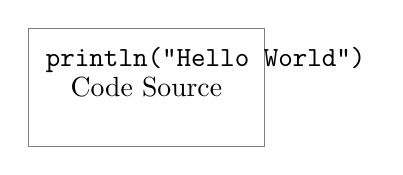
\begin{tikzpicture}
\draw[draw=gray, thin] (0,-0.5) rectangle (3,1);
\draw (0.1,0.6)  node[anchor=west] { \verb+println("Hello World")+};
\draw (1.5,0.25) node {Code Source}; 

\end{tikzpicture}

Le deuxième outil est celui qui permet d'éditer le code (les plus malins m'auront vu venir).

Comme le code s'écrit dans des fichiers textes, un simple éditeur de texte,
comme TextEdit, pourrait suffire.
Cependant les programmeurs utilisent en général des éditeurs dédiés,
qui possèdent des fonctionnalités supplémentaires, comme la coloration du code.
\begin{figure}[H]
\centering
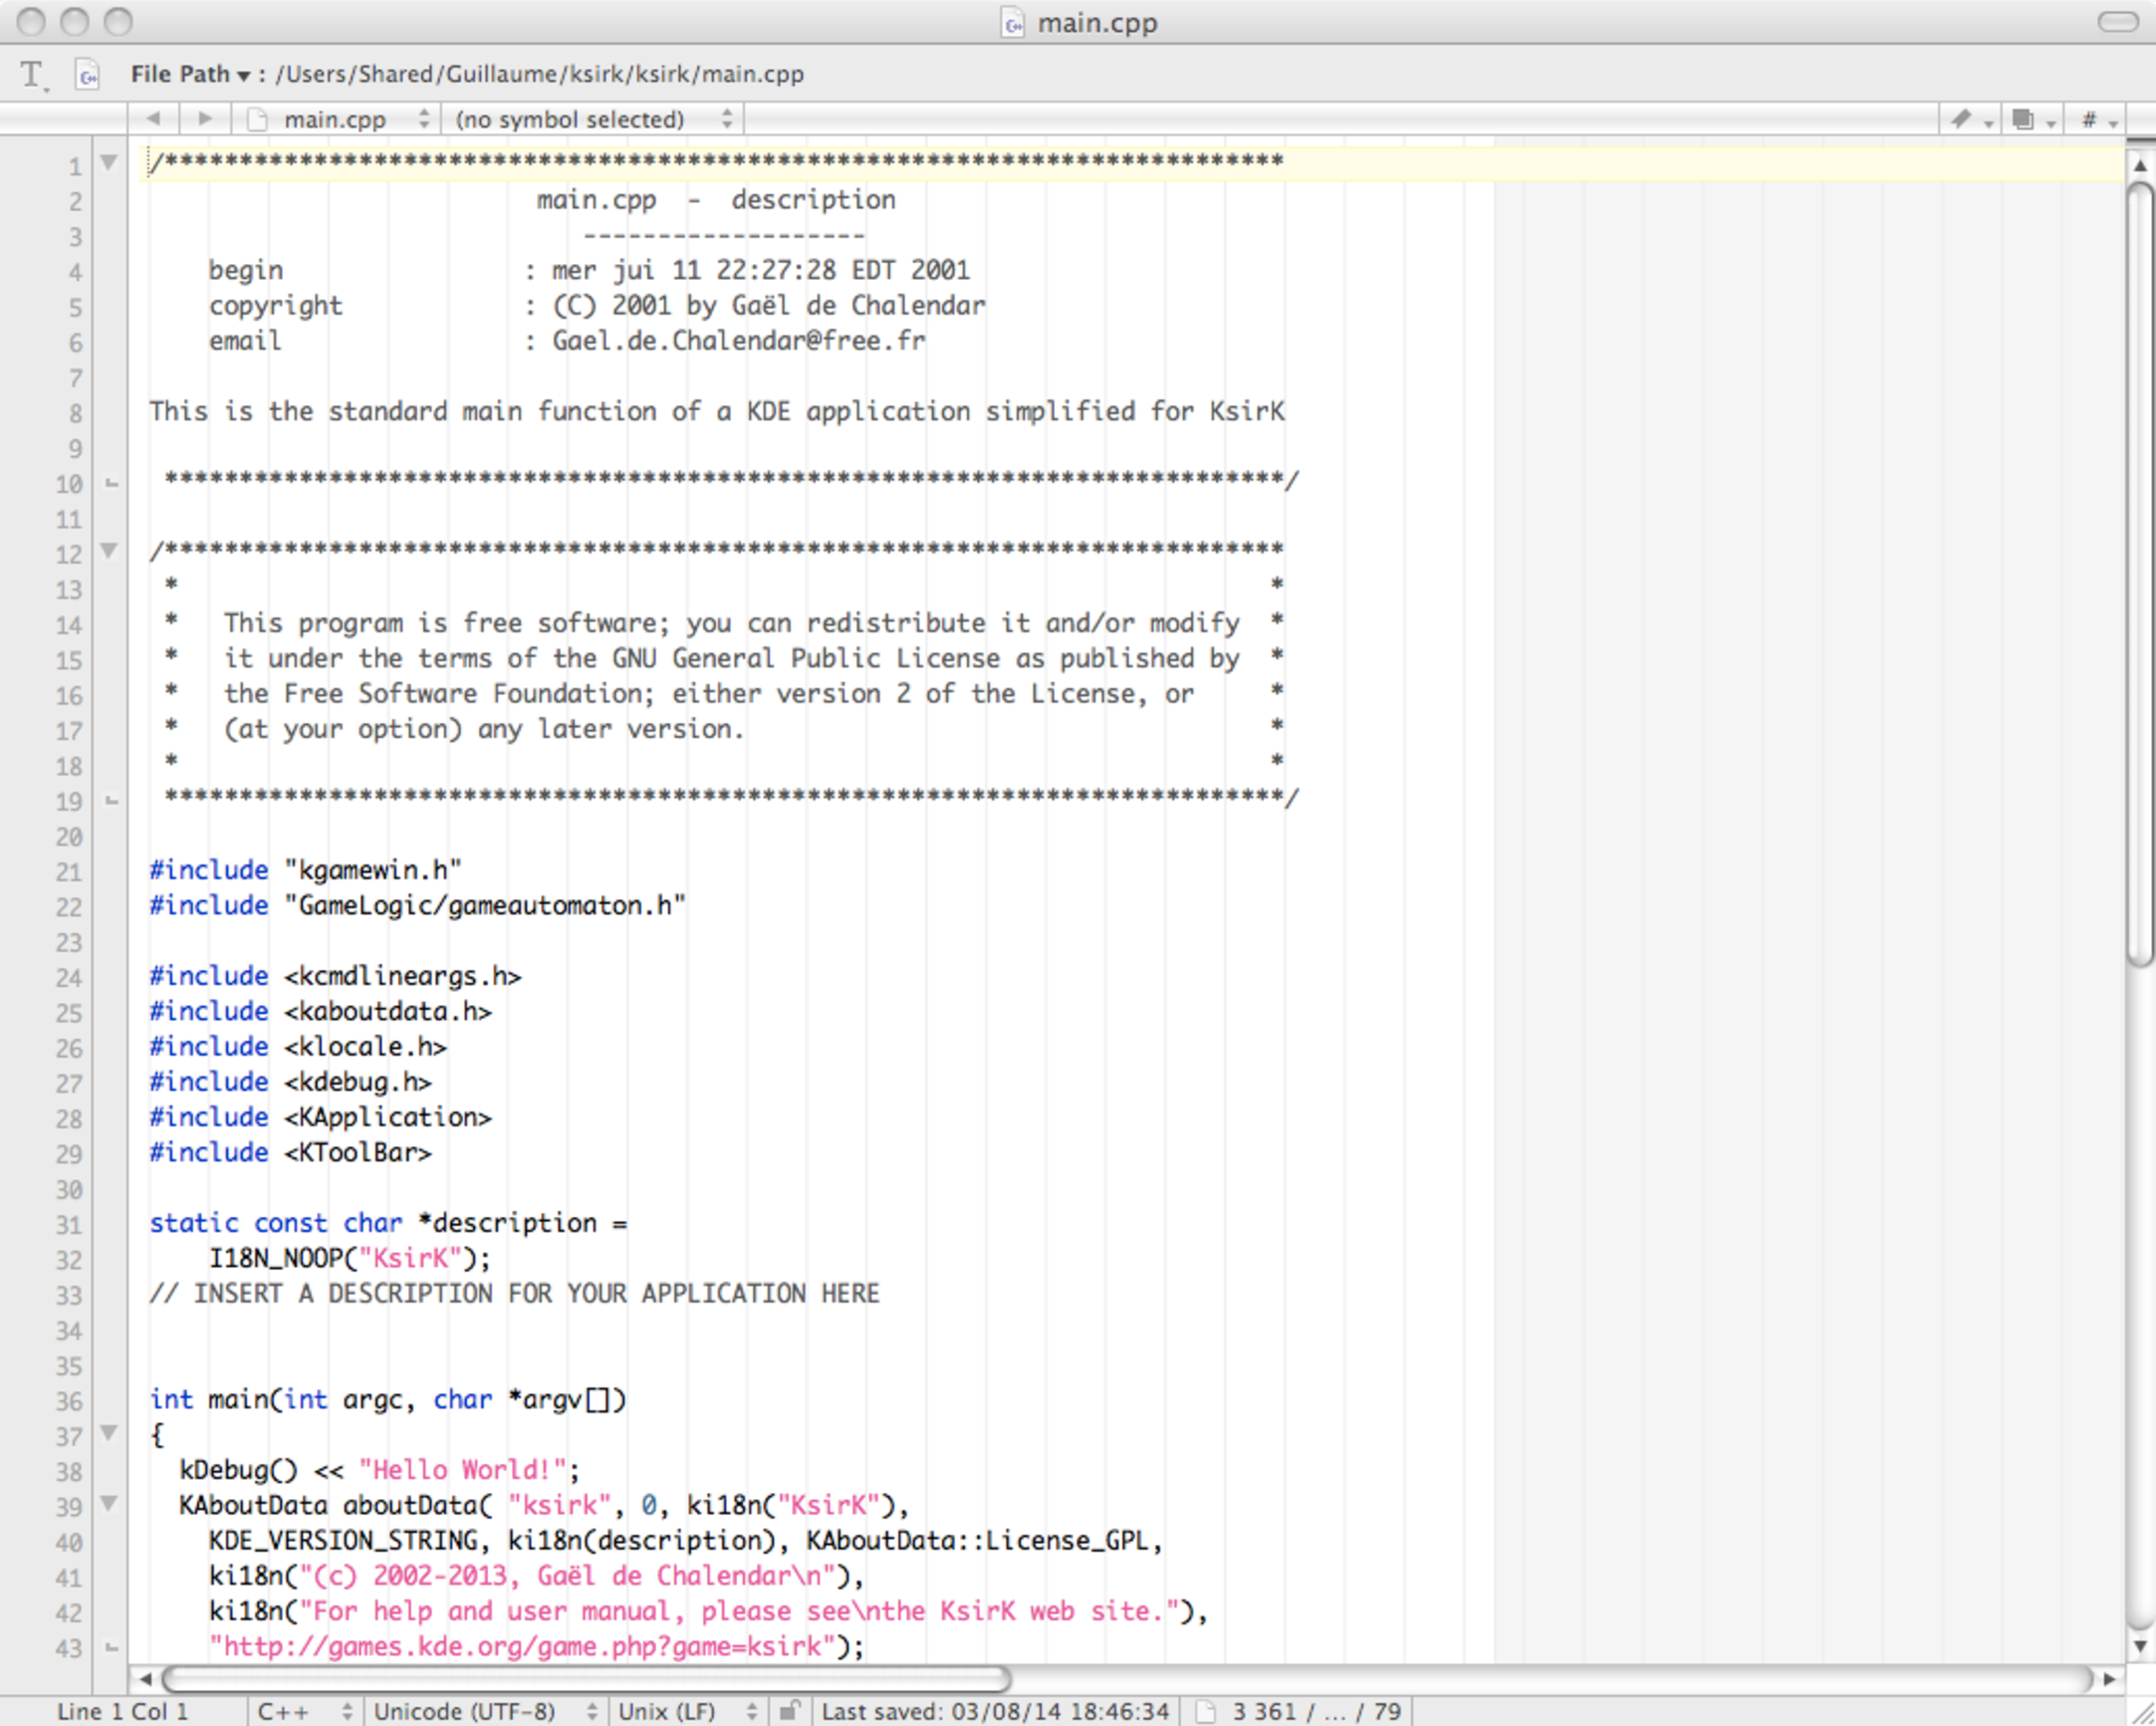
\includegraphics[scale=0.4]{\TSwiftRoot/P1-LesBasesImperatives/CH1-AvantDeCommencer/img/TextWrangler}
\caption{TextWrangler, un éditeur de text gratuit pour Mac, d'excellente facture}
\end{figure}

Enfin un troisième outil est un debugger,
qui permet de contrôler l'exécution pas à pas du programme,
en accédant aux valeurs des différentes variables,
pour comprendre ce qu'il fait,
en particulier lorsque il ne fait pas ce que l'on attend.
(En théorie, si l'on ne faisait pas d'erreur,
on pourrait s'en passer,
mais << \emph{errare humanum est.} >> )

Mais pour simplifier les choses, il a été créé un type de programme particulier,
les \emph{IDE, Environnements de Développement Intégrés},
qui regroupent ces trois fonctionnalités.
Sur Mac OS X, l'EDI fourni par Apple s'appelle \emph{Xcode},
et nous l'allons installer tout à l'heure !

\section*{Conclusion}
\phantomsection
\addcontentsline{toc}{section}{Conclusion}
Dans cette partie vous avez appris :
\begin{itemize}
\item Comment lire et travailler ce cours.
\item Ce qu'est un ordinateur.
\item Comment on peut se faire comprendre d'un ordinateur,
ou ce qu'est la programmation.
\item Quels sont les outils nécessaires pour programmer.
\end{itemize}
